%----------------------------------------------------------------------------------------
%	PART II
%----------------------------------------------------------------------------------------

\part{Nyxian Taxonomies}

%----------------------------------------------------------------------------------------
%	Galaxies
%----------------------------------------------------------------------------------------

\chapterimage{placeholder.png} % Chapter heading image

\chapter{Galaxies [IMAGES]}

\section{Nyxophora}

\lipsum[1-5]

\newpage
\begingroup
\thispagestyle{empty}
\begin{tikzpicture}[remember picture,overlay]
	\coordinate [below=12cm] (midpoint) at (current page.north);
	\node at (current page.north west)
	{\begin{tikzpicture}[remember picture,overlay]
			\node[anchor=north west,inner sep=0pt] at (0,0) {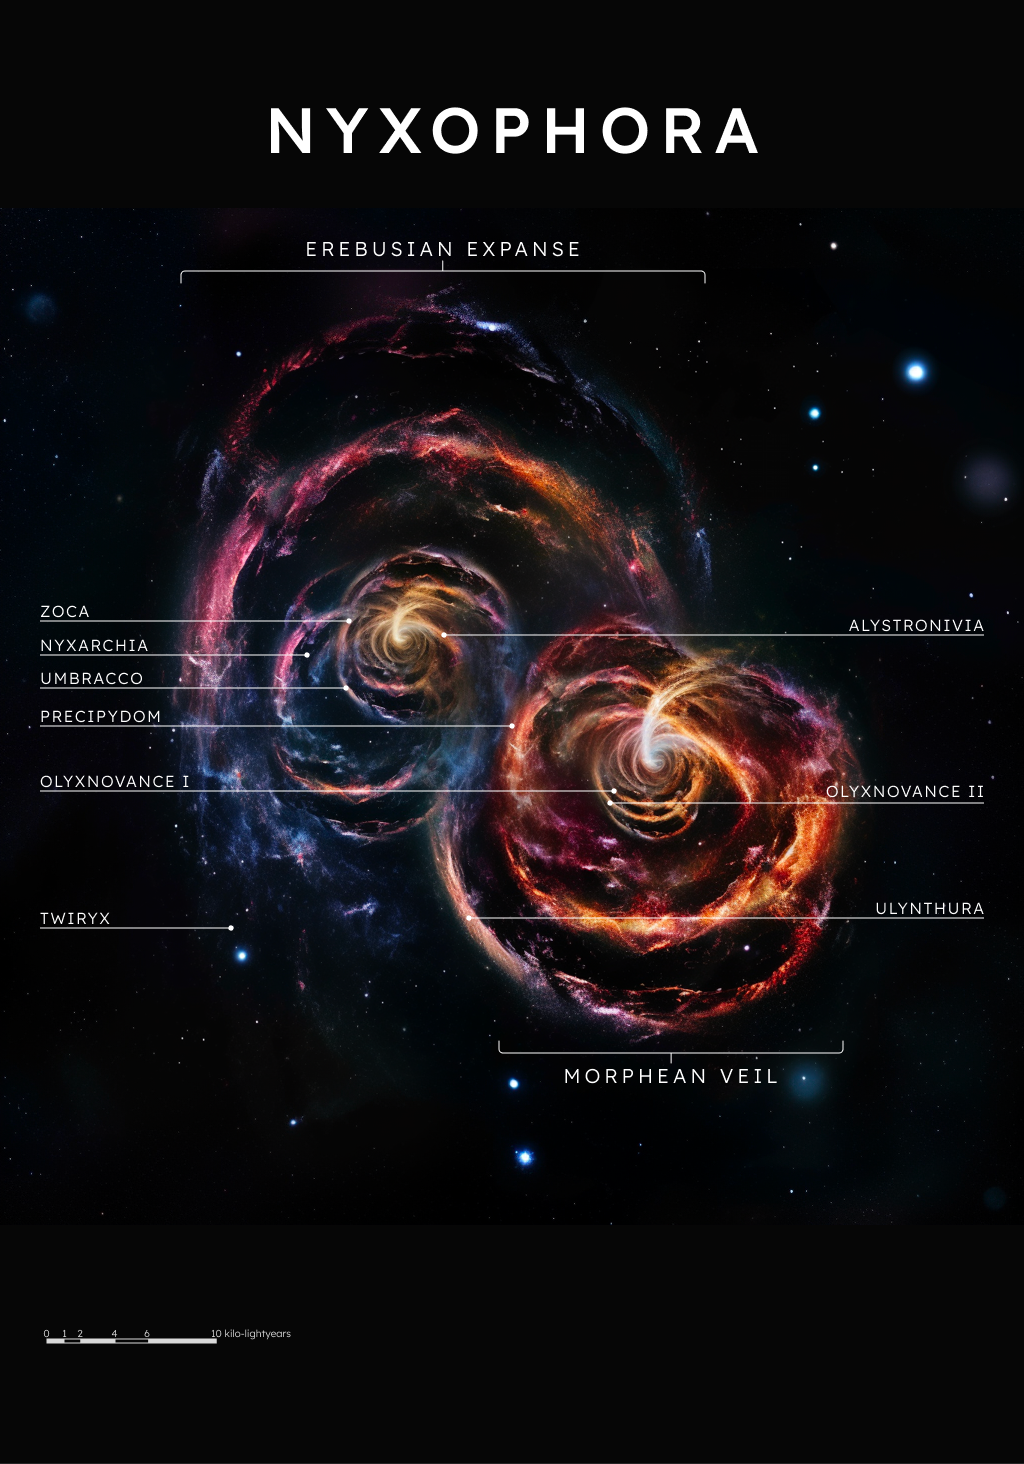
\includegraphics[width=\paperwidth]{images/pages/Nyxophora.png}}; % Background image
		\end{tikzpicture}};
\end{tikzpicture}
\vfill
\endgroup
\newpage

\section{Nyxophora: Nyxarchia}

\lipsum[6-8]

\newpage
\begingroup
\thispagestyle{empty}
\begin{tikzpicture}[remember picture,overlay]
	\coordinate [below=12cm] (midpoint) at (current page.north);
	\node at (current page.north west)
	{\begin{tikzpicture}[remember picture,overlay]
			\node[anchor=north west,inner sep=0pt] at (0,0) {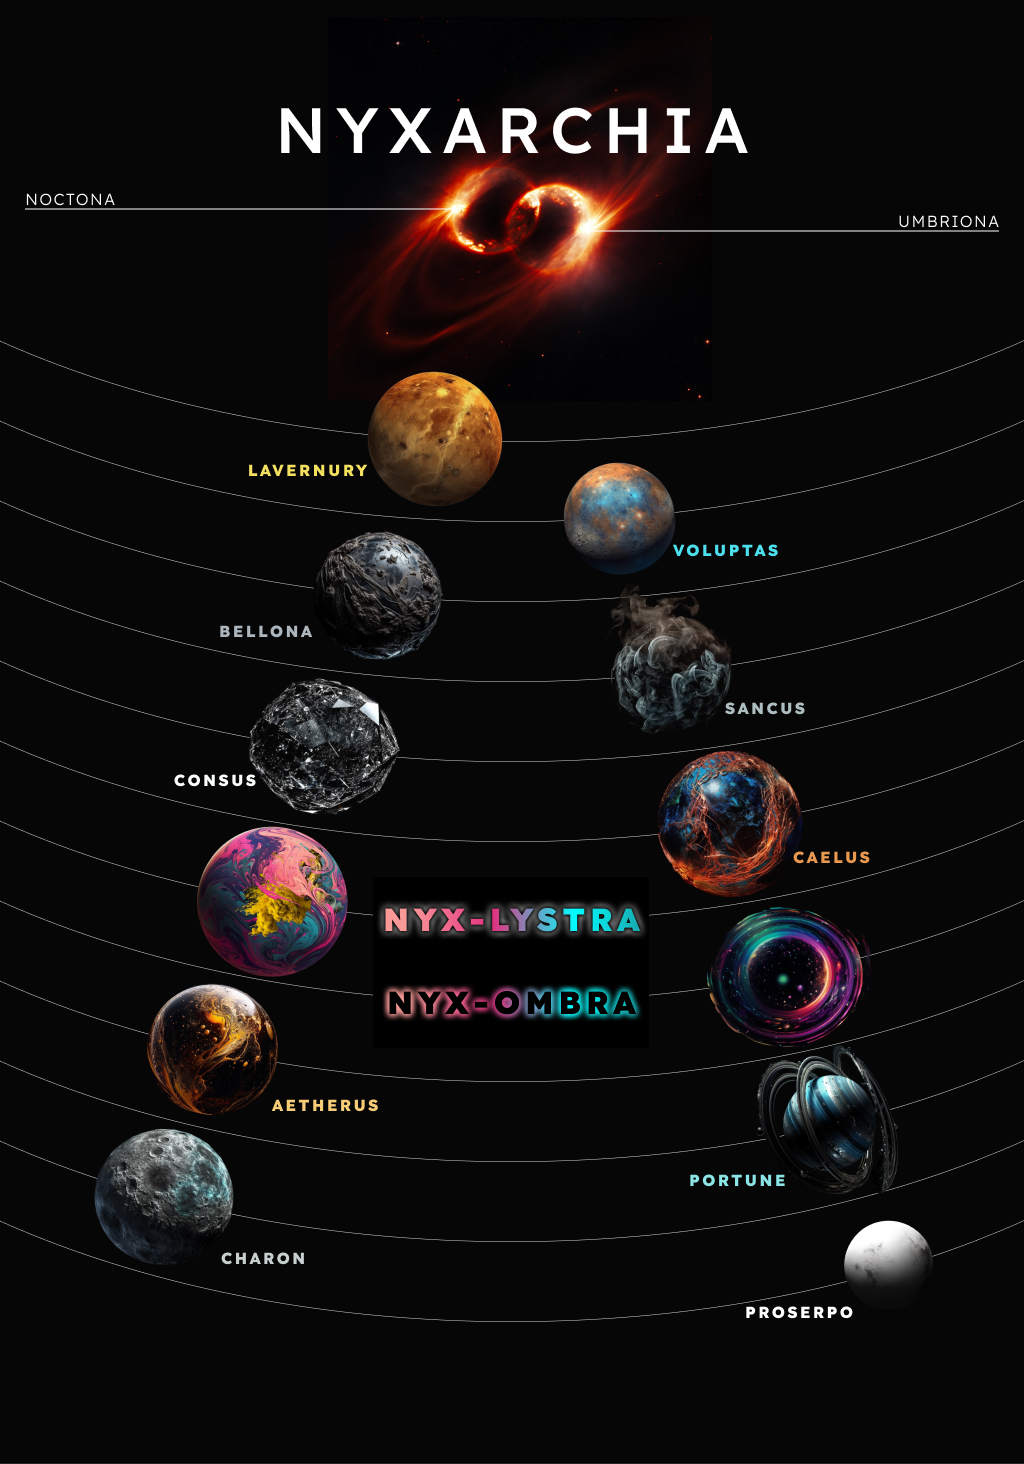
\includegraphics[width=\paperwidth]{images/pages/Nyxarchia.png}}; % Background image
		\end{tikzpicture}};
\end{tikzpicture}
\vfill
\endgroup
\newpage

\section{Fyunisai}

%----------------------------------------------------------------------------------------
%	CHAPTER
%----------------------------------------------------------------------------------------

\chapterimage{placeholder.png} % Chapter heading image

\chapter{The Nyxian Worlds [TODO]}

%----------------------------------------------------------------------------------------
%	CHAPTER
%----------------------------------------------------------------------------------------

\chapterimage{placeholder.png} % Chapter heading image

\chapter{Physiology [IMAGES]}

\section{Biology}

The Nyxi are

\section{Clades}

\subsection{Fadiglaux}

\begin{wrapfigure}{L}{0.4\textwidth}
	\centering
	
\includegraphics[width=0.38\textwidth]{clades/Fadiglaux.png}
\end{wrapfigure}

\lipsum[1]

\subsection{Baroquinfernum}

\begin{wrapfigure}{R}{0.4\textwidth}
	\centering
	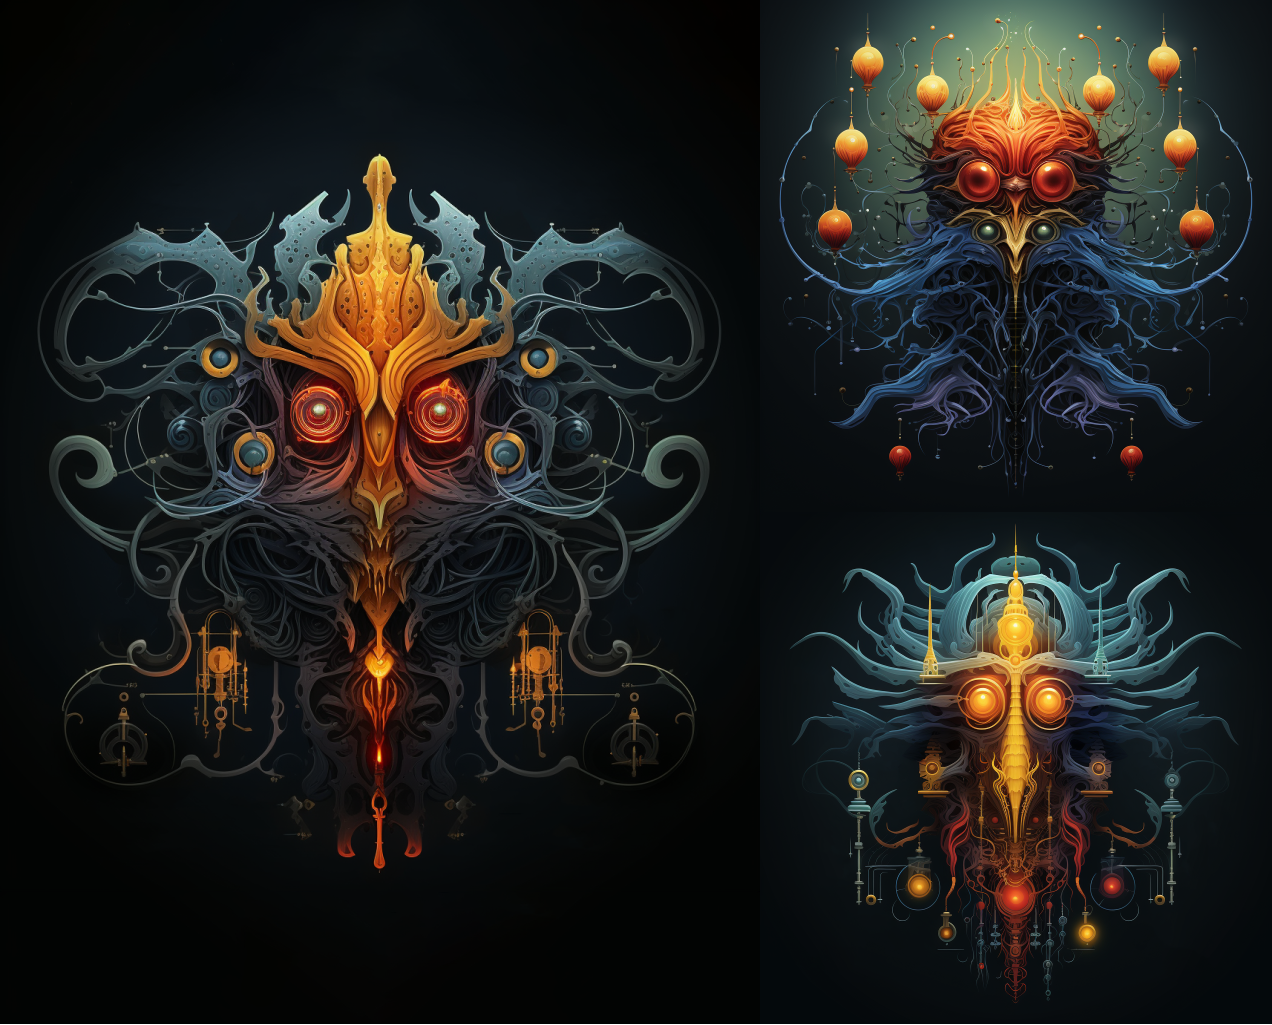
\includegraphics[width=0.38\textwidth]{clades/Baroquinfernum.png}
\end{wrapfigure}

\lipsum[2]

\subsection{Vanitavix}

\begin{wrapfigure}{L}{0.4\textwidth}
	\centering
	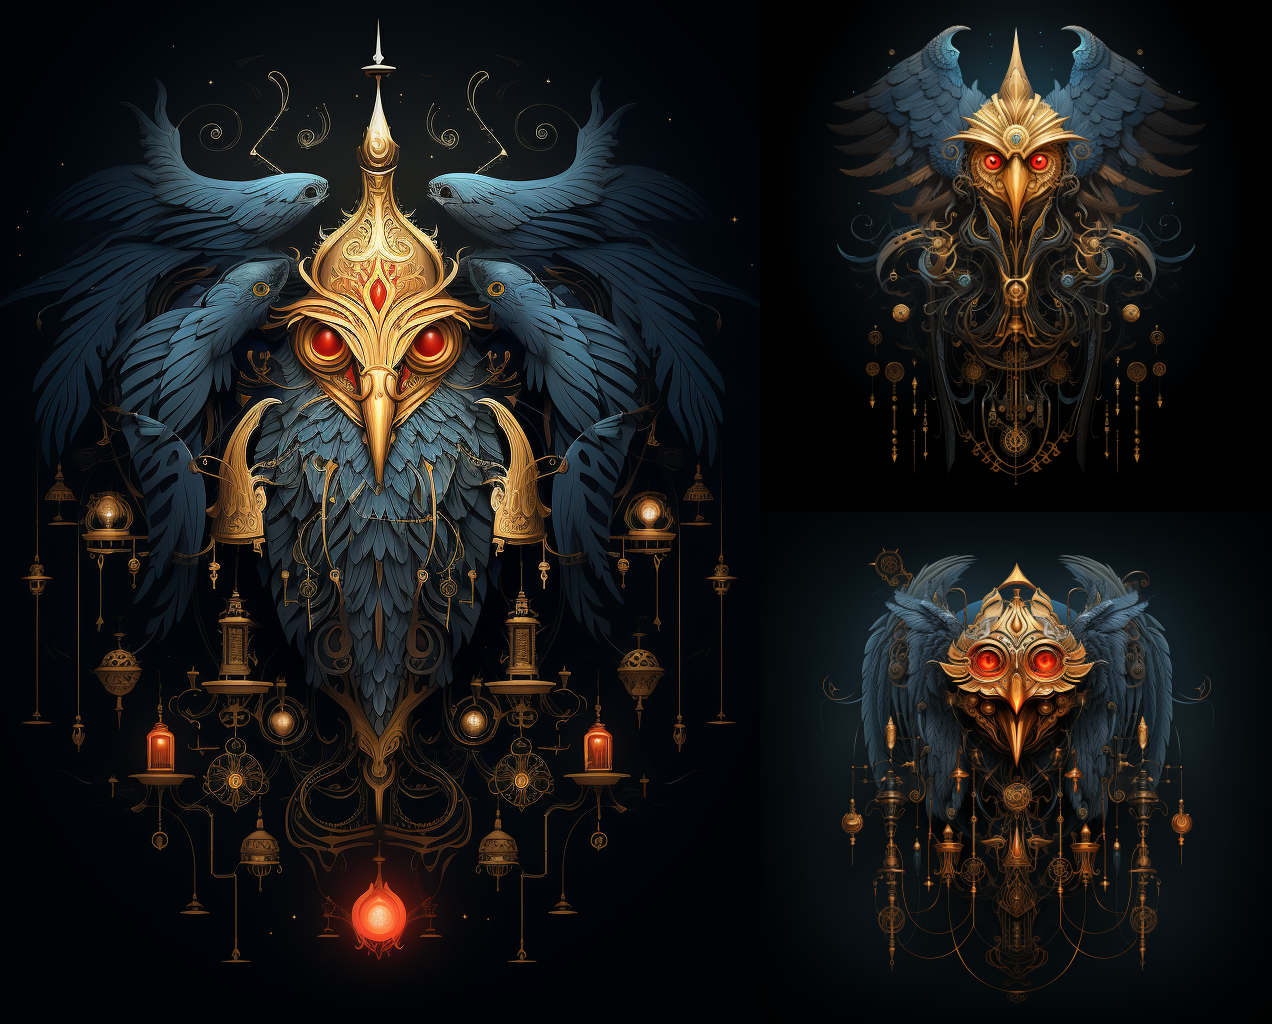
\includegraphics[width=0.38\textwidth]{clades/Vanitavix.png}
\end{wrapfigure}

\lipsum[3]

\subsection{Psychenyctua}

\begin{wrapfigure}{R}{0.4\textwidth}
	\centering
	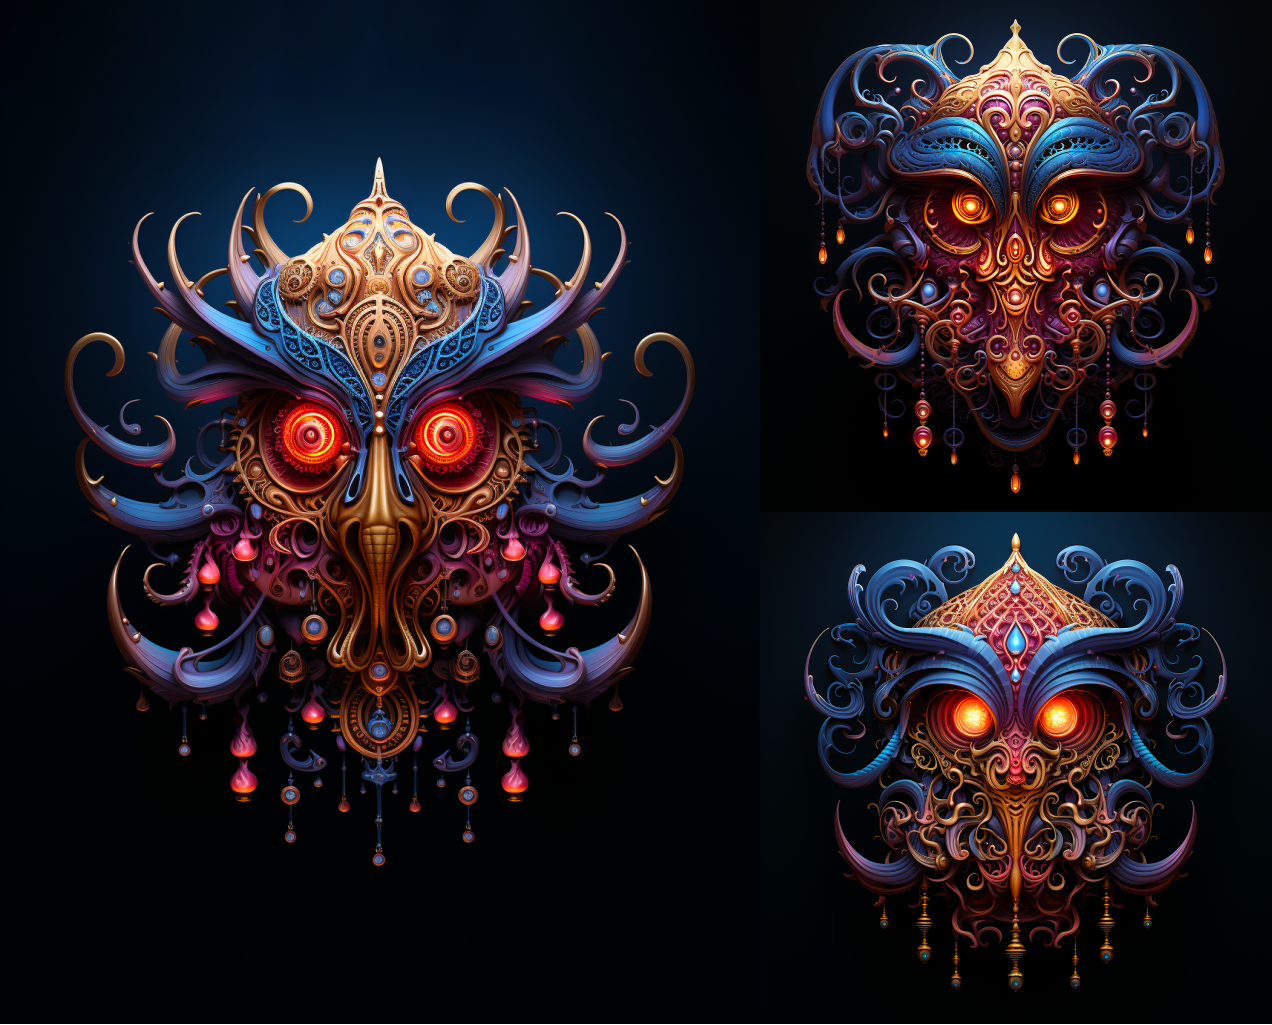
\includegraphics[width=0.38\textwidth]{clades/Psychenyctua.png}
\end{wrapfigure}

\lipsum[4]

\subsection{Sarkanagos}

\begin{wrapfigure}{L}{0.4\textwidth}
	\centering
	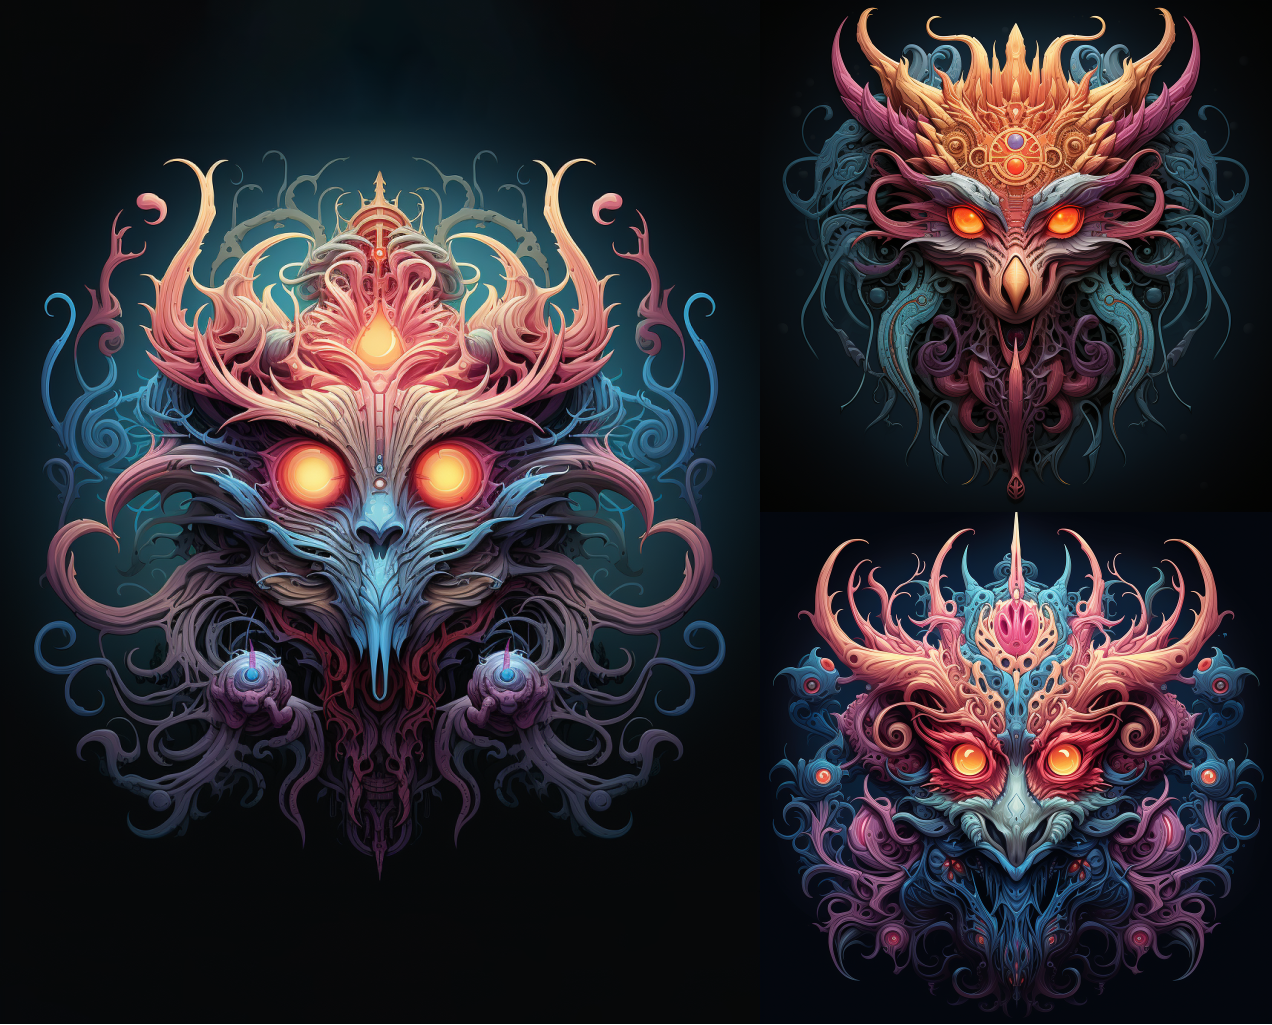
\includegraphics[width=0.38\textwidth]{clades/Sarkanagos.png}
\end{wrapfigure}

\lipsum[5]

\subsection{Ornatomedusa}

\begin{wrapfigure}{L}{0.4\textwidth}
	\centering
	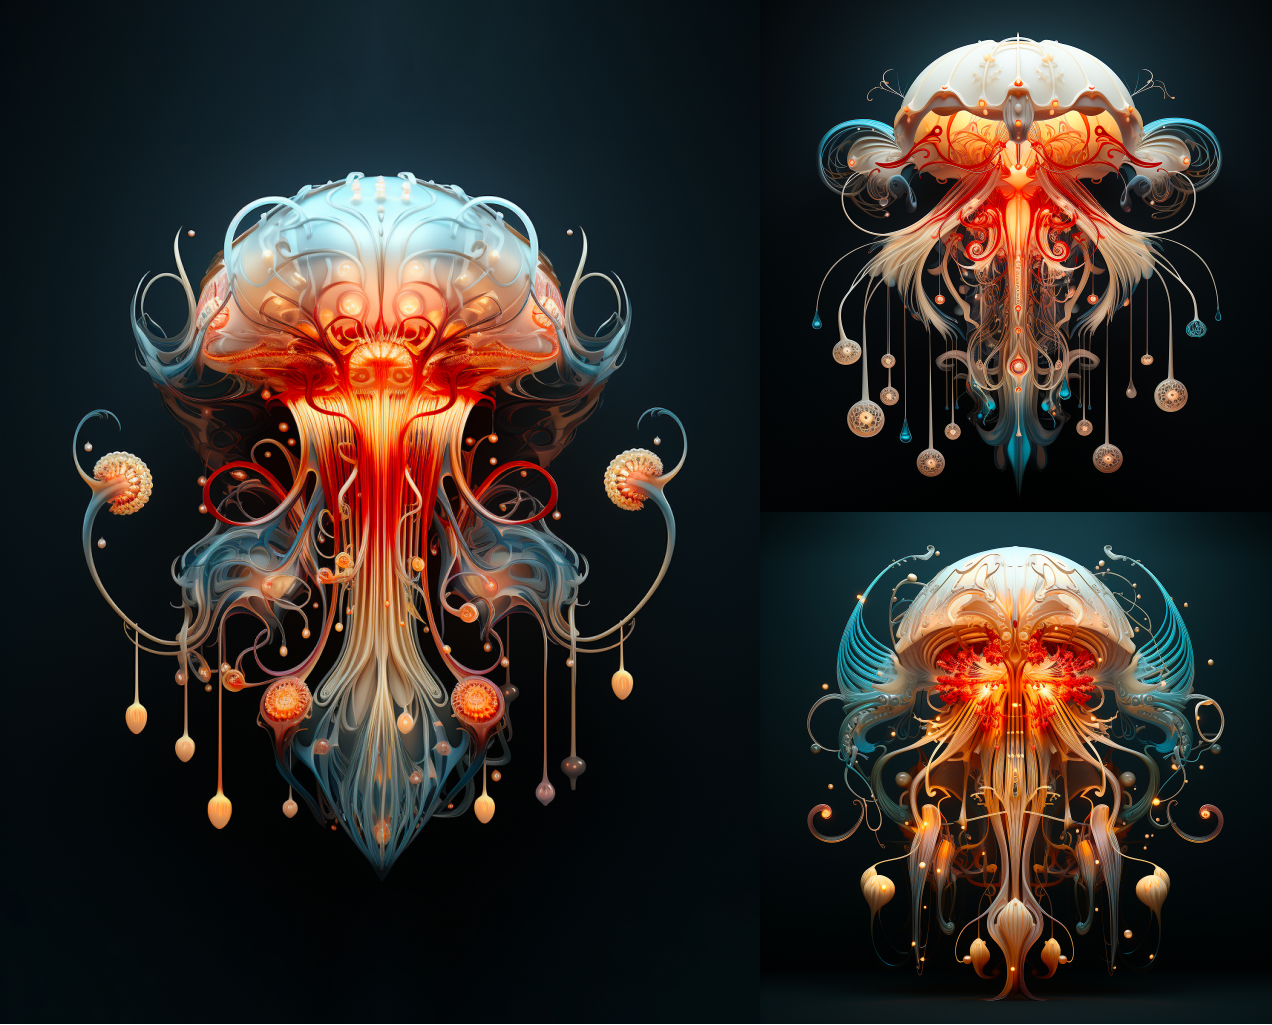
\includegraphics[width=0.38\textwidth]{clades/Ornatomedusa.png}
\end{wrapfigure}

\lipsum[6]

\subsection{Vakralakasha}

\begin{wrapfigure}{R}{0.4\textwidth}
	\centering
	
\includegraphics[width=0.38\textwidth]{clades/Vakralakasha.png}
\end{wrapfigure}

\lipsum[6]